\documentclass[12pt]{article}
\usepackage{graphicx}
\graphicspath{{imgs/}}
\usepackage{xeCJK}
\setCJKmainfont{Noto Serif CJK TC}
\usepackage[top=2cm, bottom=2cm, left=2cm, right=2cm, a4paper]{geometry}
\usepackage{setspace}
\setlength{\parskip}{2pt}
\usepackage{moresize}
\usepackage{placeins}
\usepackage{indentfirst}
\usepackage{amsmath}
\usepackage{caption, subcaption}

\begin{document}

\begin{center}
    \huge \textbf{EDA Final Project Report}
    
    \vspace{10pt}
    
    \large \textbf{110511010 楊育陞 110511067 葉哲伍}
\end{center}

\section{ICCAD 繳交截圖}

\section{Introduction}

\indent We take the \textbf{problem B} of the ICCAD contest as our final project. The problem is "Power and Timing Optimization Using Multibit Flip-Flop". Our method to solve this problem is mainly based on \textbf{clustering} and \textbf{gain-based greedy algorithm}. The clustering algorithm we use is inspired by the "Effective Mean Shift Algorithm" described in the paper "Graceful Register Clustering by Effective Mean Shift Algorithm for Power and Timing Balancing" \cite{jiang}.

\section{Method}

\subsection{Flowchart}

\begin{figure}[htbp]
    \centering
    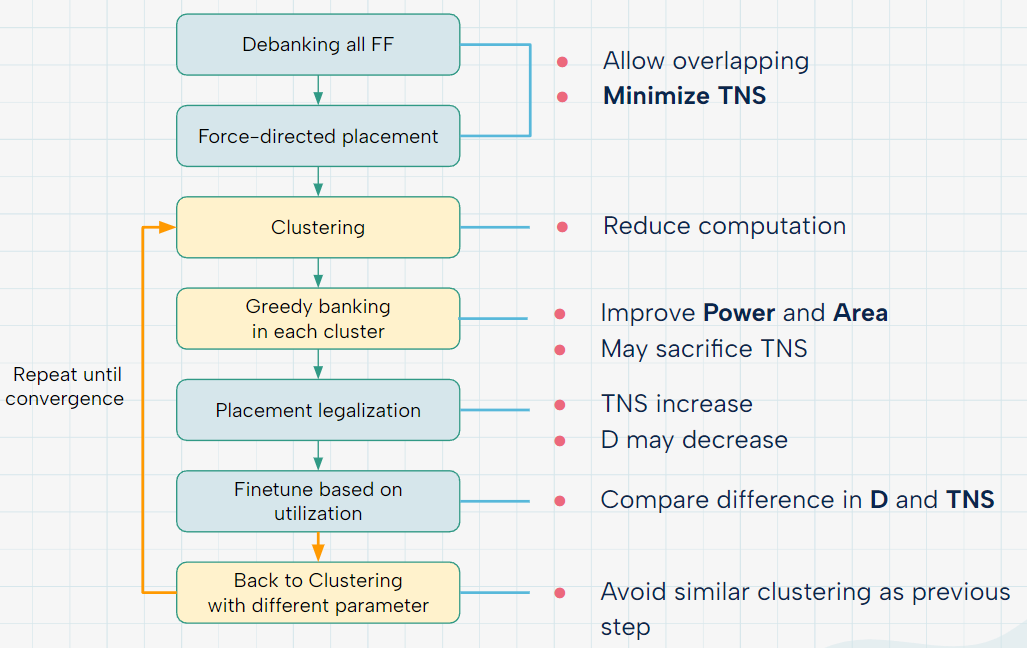
\includegraphics[width=0.9\textwidth]{flowchart2.png}
    \caption{Flowchart of our method}
    \label{fig:flowchart}
\end{figure}
\FloatBarrier

\subsection{Division of Labor}
\begin{itemize}
    \item 楊育陞: Debanking, Greedy banking, Finetuning based on utilzation
    \item 葉哲伍: Force-directed placement, Clustering, Placement legalization
\end{itemize}

\subsection{Detailed Explanation}

Our flow of the method is shown in Figure \ref{fig:flowchart}. We will explain each step in detail in the following subsections.

\subsubsection{Debanking all flip-flops}
In the initial given circuit, there are flip-flops of different bit-widths and different types. We first debank all flip-flops to single-bit flip-flops. The type of the single-bit flip-flop, called \textbf{base flip-flop} in our method, is chosen to be the single-bit flip-flop with the least cost calculated by the given cost function. The timing part of the cost is calculated by the q pin delay of the flip-flop in this step.

The debanking process is shown in Figure \ref{fig:debanking}. The debanked flip-flops are placed in the same position as the original flip-flops, and the connections are also kept the same. In this step, we allow the cells to overlap with each other.

\begin{figure}[htbp]
    \centering
    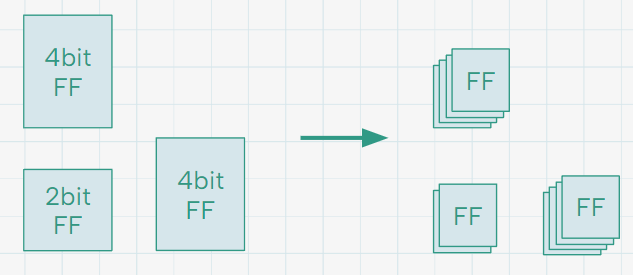
\includegraphics[width=0.7\textwidth]{debank.png}
    \caption{Debanking process}
    \label{fig:debanking}
\end{figure}

\subsubsection{Force-directed placement}

\subsubsection{Clustering}

\subsubsection{Greedy banking in each cluster}

\subsubsection{Placement legalization}

\subsubsection{Finetuning based on utilization}

\subsubsection{Back to clustering with different parameters}

\section{Result}

\section{Conclusion}

\begin{thebibliography}{9}
    \bibitem{jiang} 
    Ya-Chu Chang, Tung-Wei Lin, Iris Hui-Ru Jiang, and GiJoon Nam. "Graceful Register Clustering by Effective Mean Shift Algorithm for Power and Timing Balancing." Proceedings of the 2019 International Symposium on Physical Design (ISPD '19), 2019.
\end{thebibliography}

\end{document}
